\documentclass[pdflatex,compress]{beamer}

%\usetheme[dark,framenumber,totalframenumber]{ElektroITK}
\usetheme[darktitle,framenumber,totalframenumber]{ElektroITK}
\usepackage[utf8]{inputenc}
\usepackage[T1]{fontenc}
\usepackage{lmodern}
%\usepackage[bahasai]{babel}
\usepackage{amsmath}
\usepackage{amsfonts}
\usepackage{amssymb}
\usepackage{graphicx}
\usepackage{multicol}
\usepackage{lipsum}
\usefonttheme[onlymath]{serif}

\newcommand*{\Scale}[2][4]{\scalebox{#1}{$#2$}}%

\setbeamertemplate{caption}[numbered]

\AtBeginSection[]{
	\begin{frame}
		\vfill
		\centering
		\usebeamerfont{title}\insertsectionhead\par%
		\vfill
	\end{frame}
}

\title{Electronic Circuit II}
\subtitle{Amplifier}
\author{Mifta Nur Farid}
\date{9 March 2023}

\begin{document}

\maketitle

\begin{frame}
	\frametitle{Operational Amplifier}
	(a) Schematic symbol for op amp; (b) equivalent circuit of op amp. 
	\begin{center}
		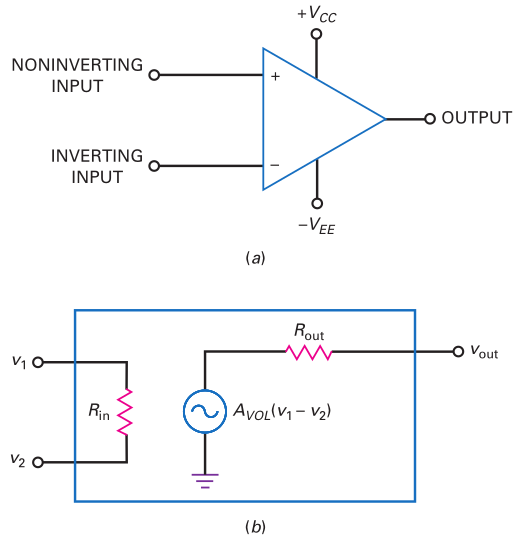
\includegraphics[width=0.4\linewidth]{img/fig1602}
	\end{center}
	$R_{in} = \infty$, $R_{out} = 0$, $A_{VOL} = \infty$.
\end{frame}

\begin{frame}
	\frametitle{Inverting Amplifier}
	\begin{center}
		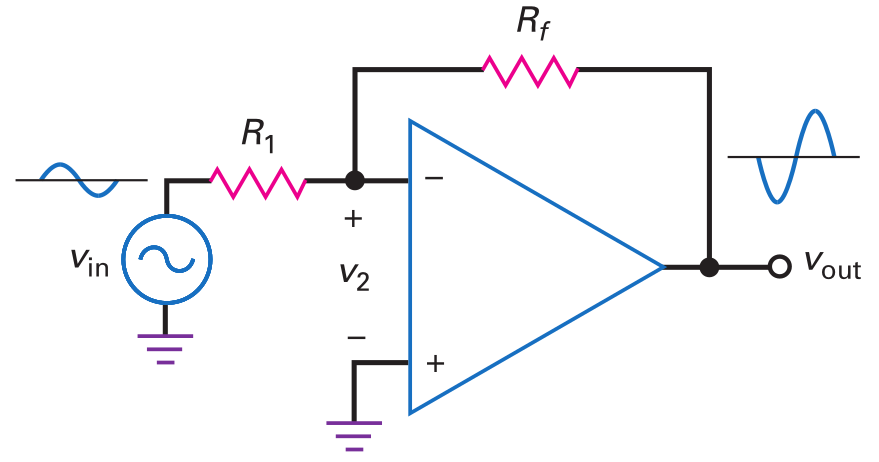
\includegraphics[width=0.7\linewidth]{img/fig1612}
	\end{center}
\end{frame}

\begin{frame}
	\frametitle{Inverting Amplifier - Virtual Ground}
	The concept of virtual ground: shorted to voltage and open to current.
	\begin{multicols}{2}
		\begin{center}
			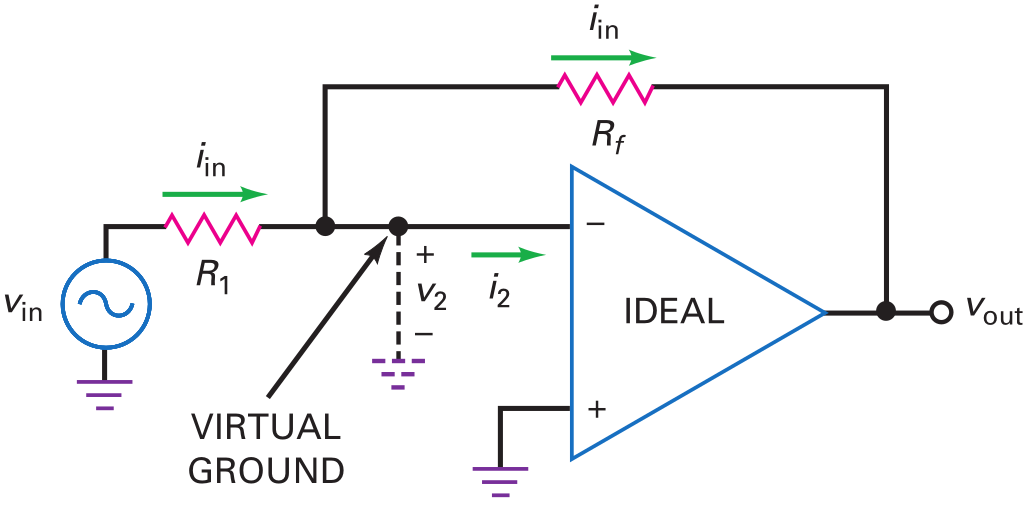
\includegraphics[width=\linewidth]{img/fig1613}
		\end{center}
		\columnbreak
		\begin{itemize}
			\item $R_{in} = \infty \rightarrow i_2 = 0$
			\item $A_{VOL} = \infty \rightarrow v_2 = 0$
			\item the inverting input acts like a ground for voltage but an open for current
		\end{itemize}
	\end{multicols}
\end{frame}

\begin{frame}
	\frametitle{Inverting Amplifier - Voltage Gain}
	Inverting amplifier has same current through both resistors.
	\begin{multicols}{2}
		\begin{center}
			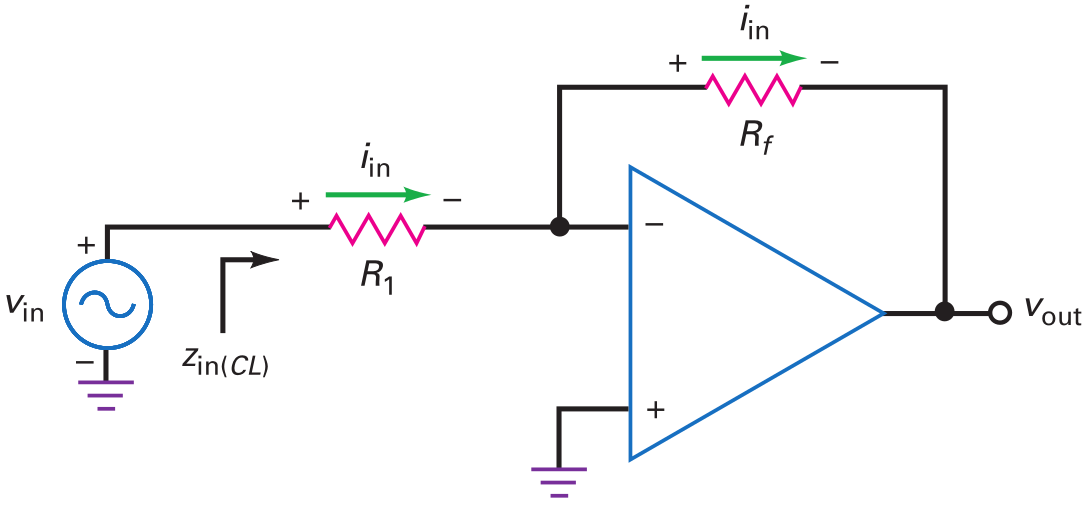
\includegraphics[width=\linewidth]{img/fig1614}
		\end{center}
		\columnbreak
		\begin{itemize}
			\item $v_{in} = i_{in} R_1$
			\item $v_{out} = -i_{in} R_f$
			\item $A_V = v_{out} / v_{in} = -i_{in} R_f / i_{in} R_1$
			\item $A_{V(CL)} = \frac{-R_f}{R_1}$
		\end{itemize}
	\end{multicols}
	
\end{frame}


\begin{frame}
	\frametitle{Nonnverting Amplifier}
	\begin{center}
		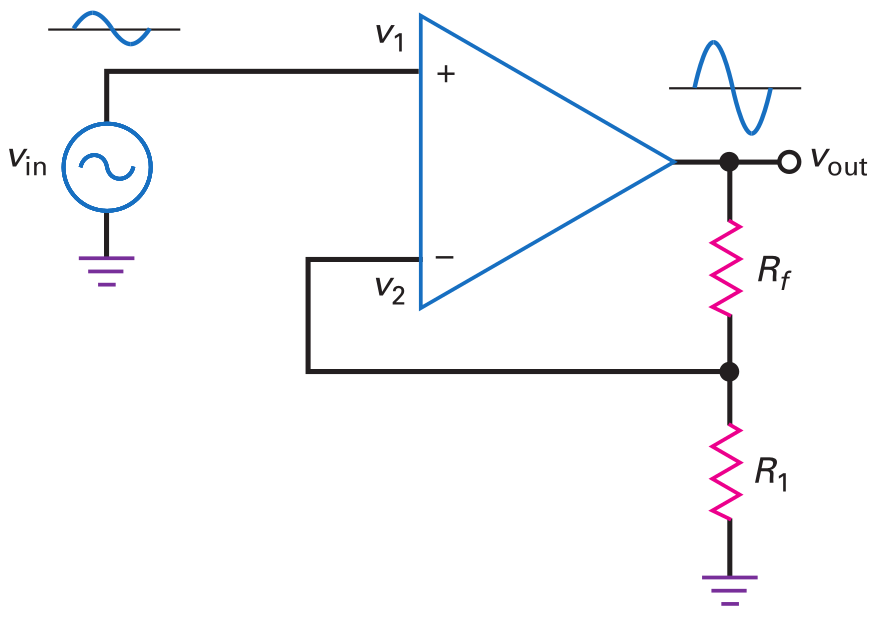
\includegraphics[width=0.7\linewidth]{img/fig1618}
	\end{center}
\end{frame}

\begin{frame}
	\frametitle{Noninverting Amplifier - Virtual Short}
	The virtual short is a short for voltage but an open for current.
	\begin{multicols}{2}
		\begin{center}
			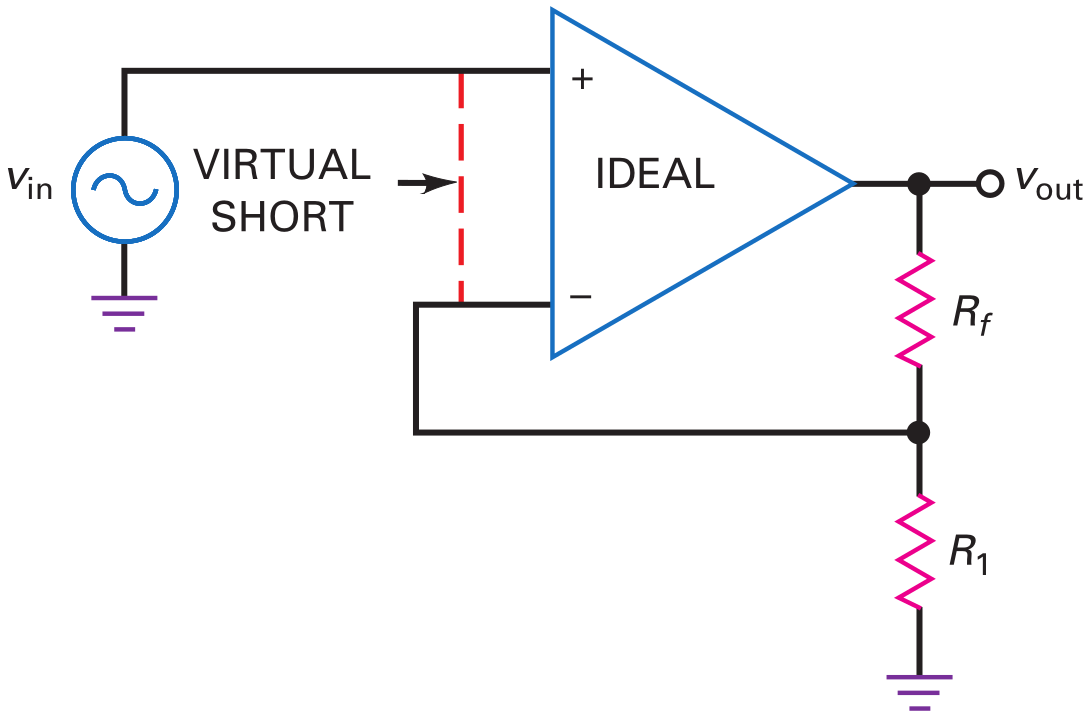
\includegraphics[width=\linewidth]{img/fig1619}
		\end{center}
		\columnbreak
		\begin{itemize}
			\item $R_{in} = \infty \rightarrow \text{ both } i_{in} = 0$
			\item $A_{VOL} = \infty \rightarrow v_1 - v_2 = 0$
		\end{itemize}
	\end{multicols}
\end{frame}

\begin{frame}
	\frametitle{Noninverting Amplifier - Voltage Gain}
	Input voltage appears across R1 and same current flows through resistors.
	\begin{multicols}{2}
		\begin{center}
			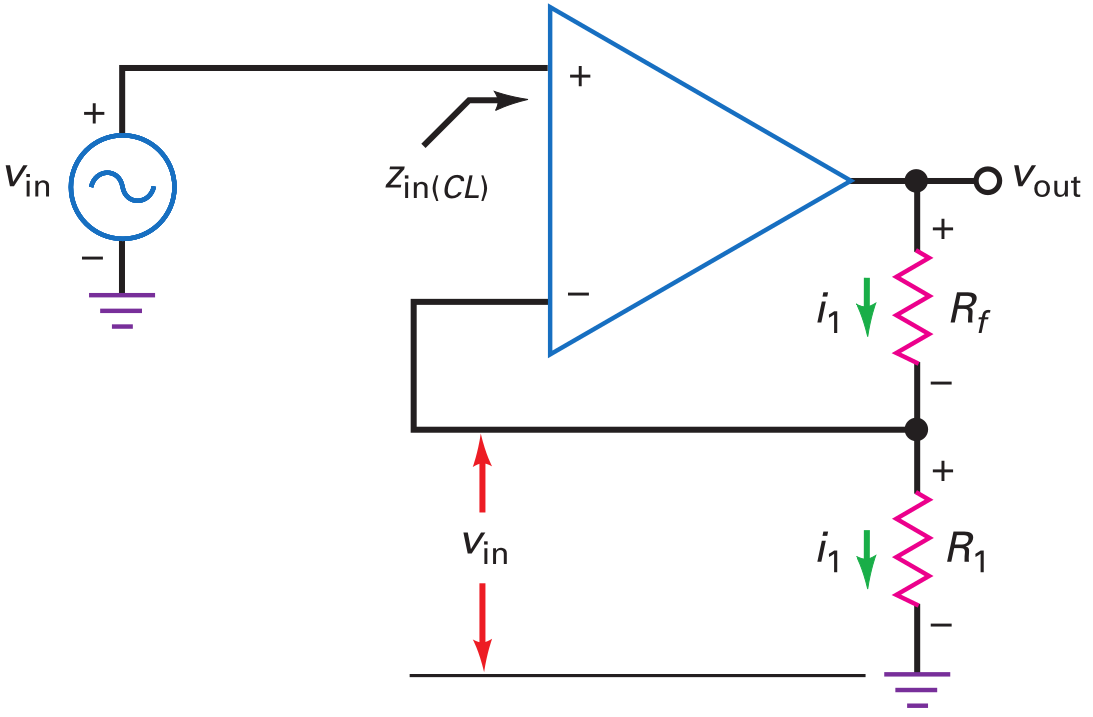
\includegraphics[width=0.7\linewidth]{img/fig1620}
		\end{center}
		\columnbreak
		\begin{itemize}
			\item $v_{in} = i_1 R_1$
			\item $v_{out} = i_1 (R_f + R_1)$
			\item $A_{V(CL)} = \frac{R_f + R_1}{R_1} = \frac{R_f}{R_1} + 1$
		\end{itemize}
	\end{multicols}
\end{frame}

\begin{frame}
	\frametitle{Summing Amplifier}
	\begin{center}
		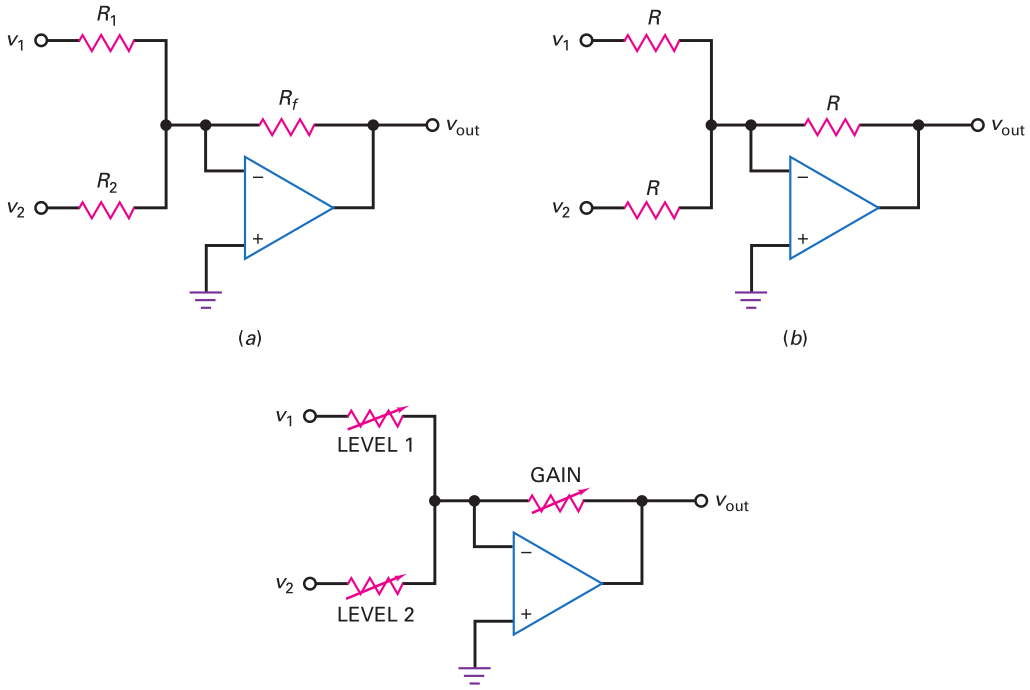
\includegraphics[width=\linewidth]{img/fig1623}
	\end{center}
\end{frame}

\begin{frame}{Summing Amplifier}
	\begin{itemize}
		\item $A_{V1(CL)} = \frac{-R_f}{R_1}$
		\item $A_{V2(CL)} = \frac{-R_f}{R_2}$
		\item $v_{out} = A_{V1(CL)}v_1 + A_{V2(CL)}v_2$
	\end{itemize}
\end{frame}

\begin{frame}
	\frametitle{Summary}
	\begin{center}
		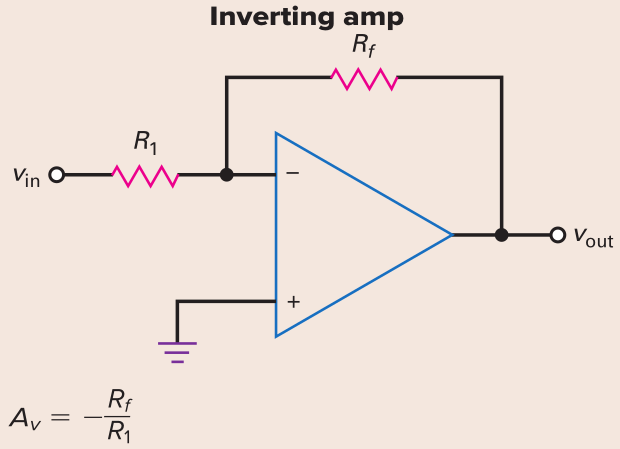
\includegraphics[width=0.7\linewidth]{img/tab1602a}
	\end{center}
\end{frame}

\begin{frame}{Summary}
	\begin{center}
		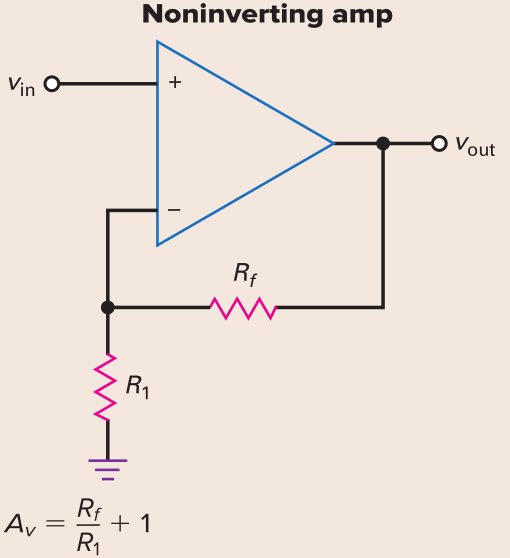
\includegraphics[width=0.6\linewidth]{img/tab1602b}
	\end{center}
\end{frame}

\begin{frame}{Summary}
	\begin{center}
		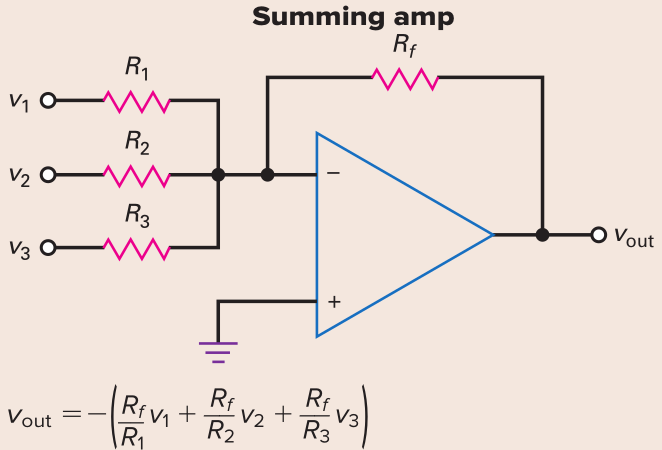
\includegraphics[width=0.7\linewidth]{img/tab1602c}
	\end{center}
\end{frame}

\end{document}
